\documentclass[letterpaper,11pt]{article}
\usepackage{graphicx}
\usepackage{listings}
\usepackage{hyperref}
\usepackage{amsmath}
\usepackage{url}
\def\UrlBreaks{\do\/\do-}
\usepackage[normalem]{ulem}
\newcommand{\tab}[1]{\hspace{.2\textwidth}\rlap{#1}}
\usepackage{xcolor}
\usepackage{sectsty}
\sectionfont{\color{blue}}
\usepackage{titlesec}
\usepackage{fancyvrb}
\usepackage{listings}
\usepackage{caption}
\usepackage[vertfit]{breakurl}
\sloppy

\titleformat{\section}
{\color{blue}\normalfont\Large\bfseries}
{\color{blue}\thesection}{1em}{}

\lstset{
        basicstyle=\footnotesize,
        breaklines=true,
}

\begin{document}

\begin{titlepage}
\begin{center}
\Huge{Assignment 7}
\\
\Large{CS595}
\\
\Large{Introduction to Web Science}
\\
\Large{Old Dominion University}
\\
\Large{Computer Science}
\\
\Large{Due: 11:59 pm Nov 7}
\\
\Large{Lulwah Alkwai}
\\
\end{center}
\end{titlepage}
\newpage

\section*{Question 1}

Using D3, create a graph of the Karate club before and after the split \\

Weight the edges with data from: \url{http://vlado.fmf.uni-lj.si/pub/networks/data/ucinet/zachary.dat} \\

Have the transition from before/after the split occur on a mouse click.  \\
\newpage

\subsection*{Answer to Question 1}
To create a D3 Karate Club graph I used the data from: \url{http://vlado.fmf.uni-lj.si/pub/networks/data/ucinet/zachary.dat} as a data input for the D3 file.\\

Also, I created to groups of nodes, which are the two groups that were created after the split. I did this in order to randomly assign positions of one group on left side and randomly position the other group to the right side. In addition, the two grouping was used in determining the colors of the group when selecting different views.\\

To toggle between before the split and after views; at first I made the nodes clickable; however I did not like the idea of searching for the exact position of the node to make it toggle between views; So alternatively I added a button that is clicked in order to switch between views.\\

You can always re-position the nodes in order to have a different view.\\

Here is a link to the graph:\\
\url{http://www.cs.odu.edu/~lalkwai/KarateClub.html}

\begin{minipage}{\linewidth}
\hspace*{-1.6in}
\fbox{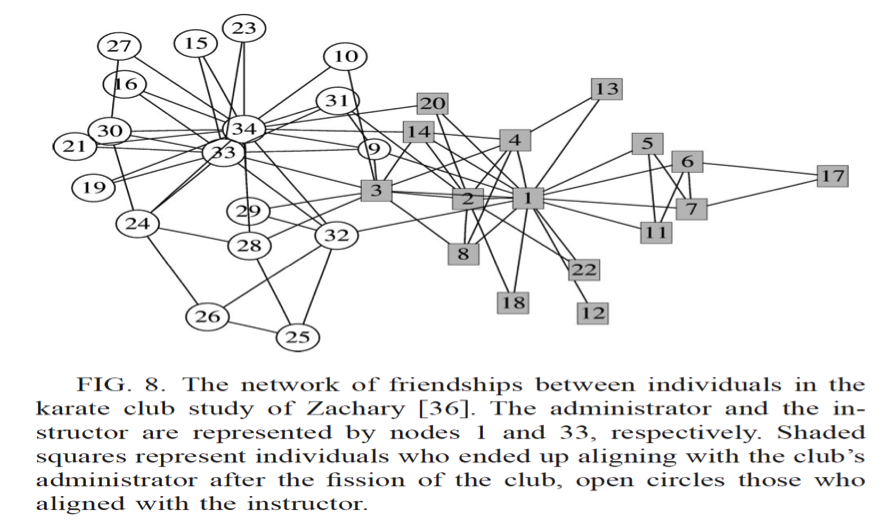
\includegraphics[keepaspectratio=true,scale=.5]{g1.png}}
\captionof{figure}{Before Split}
\label{visina8}
\end{minipage}

\begin{minipage}{\linewidth}
\hspace*{-1.6in}
\fbox{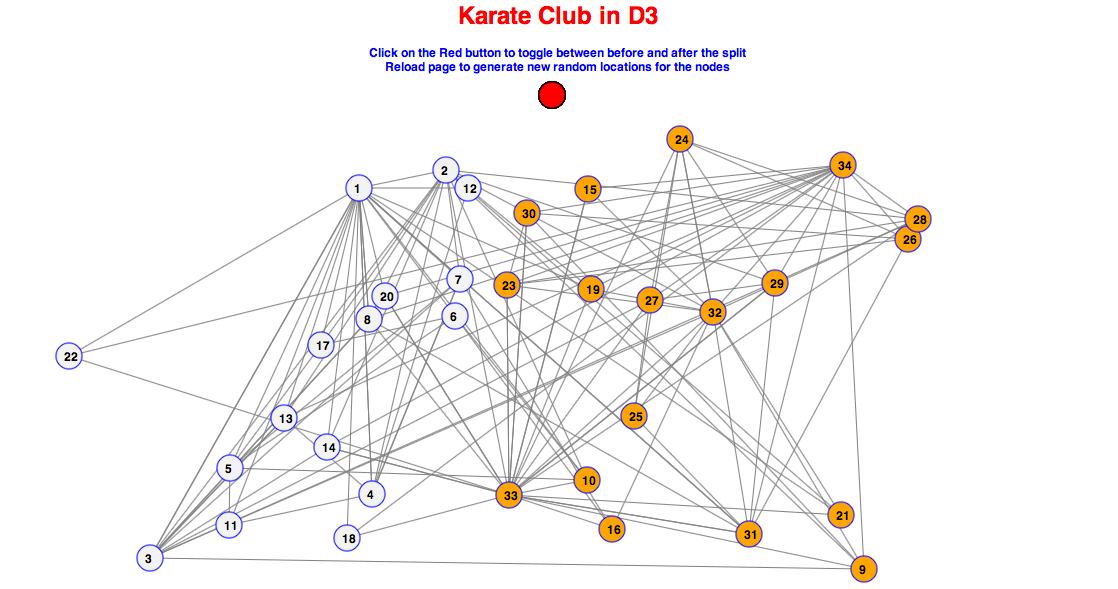
\includegraphics[keepaspectratio=true,scale=.5]{g2.png}}
\captionof{figure}{After Split}
\label{visina8}
\end{minipage}

\newpage

\section*{Extra Credit, 3 Points}

Use D3 to create a who-follows-whom graph of your Twitter account. Use my Twitter account (phonedude\_mln) if you do not have an interesting number of followers.
\newpage

\subsection*{Answer to Extra Credit}
No attempt.
\newpage

\end{document}